\chapter{Rozšiřující deska UniPi}
\label{KapUnipi}

UniPi je česká firma, nyní dceřiná společnost Faster.cz, původně její oddělení měření a regulace, která se zaměřuje na inteligentní stavební řešení, domácí automatizaci a internet věcí. Dále provozuje výzkum a vývoj rozšiřujicích desek UniPi, včetně jejich softwarového vybavení \cite{UniPiBoard}.

UniPi je taktéž pojmenování pro přídavné rozšiřující desky pro RaspberryPi, se kterou je plně kompatibilní ve všech verzích. Je vybavena řadou komponent, jako jsou například digitální galvanicky oddělené vstupy s LED signalizací, 0\,-\,10\,V analogové vstupy, 0\,-\,10\,V analogové výstupy, spínací relé, jednokanálová 1Wire sběrnice, I2C sběrnice, UART sběrnice, SPI sběrnice a RS-485 sběrnice.

UniPi je název, odvozený od slov \uv{RaspberryPi} a \uv{univerzální}, protože jednoduchost a univerzálnost jsou základní charakteristiky této desky. Deska původně vznikla pro potřeby řízení energetických hodnot vlastního datacentra Zelená Data \cite{ZelenaData}, ale škála odvětví, kde je možné UniPi nasadit je rozsáhlá, pro představu výrobce úuvádí několik příkladů \cite{UniPiBoard}:
\begin{itemize}
	\item Docházkové a přístupové systémy.
	\item Bezpečnostní systémy.
	\item Topné, chladící prvky i řízení.
	\item Větrání, rekuperace.
	\item Řídící systémy, které nejsou kompletní.
	\item Dohledové systémy.
	\item Ovládání světelných prvků.
	\item Datové vypínače.
	\item Řízení pivovarnických technologií.
	\item Zavlažovací systémy.
	\item Wellness systémy – vířivé vany, bazény, sauny.
	\item Solární systémy.
\end{itemize}

\vspace{5mm}
\noindent
 V současnosti existují dvě verze rozšiřující desky UniPi:


\begin{itemize}
	\item UniPi (verze 1)\footnote[1]{Dostupné z: http://unipi.technology/product/unipi/}.
	\item UniPi Neuron (verze 2)\footnote[2]{Dostupné z: http://unipi.technology/product/unipi-neuron-s103/}.
\end{itemize}

\vspace{5mm}
Desky se liší svými vstupně-výstupními možnostmi, rozměry a jsou dostupné v několika variantách.



%%%%%%%%%%%%%%%%%%%%%%%%%%%%%%%%%%%%%%%
%%%%%%%%%%%%%%%%%%%%%%%%%%%%%%%%%%%%%%%
%%%%%%%%%%%%%%%%%%%%%%%%%%%%%%%%%%%%%%%

\section{UniPi v1}
\label{KapitolaUnipi1}

Deska UniPi je prezentována jako nejlevnější a nejjednodušší řešení pro inteligentní budovy a IoT. Deska je navržena pro maximální kompatibilitu s mini počítačem RaspberryPi, který se dnes dá pořídit již za několik stokorun.  Zařízení bylo vyvinuto primárně jako rozhraní pro příjem vstupních signálů, jejich vyhodnocení a realizaci výstupní reakce na základě naprogramovaných algoritmů \cite{UniPiBoard1}.

Disponuje osmi relé pro střídavý proud, čtrnácti digitálními vstupy, jedním jednokanálovým 1Wire rozhraním, dvěma 0\,-\,10\,V analogovými vstupy a jedním 0\,-\,10\,V analogovým výstupem. Zajímavou součástí desky je také modul reálného času. Druhý I2C port na RaspberryPi v sobě navíc ukrývá 5\,V měnič napětí a ochranu ESD (ElectroStatic Discharge), umožňující tak připojení dalších zařízení. Pro jednoduché připojení jednotlivých sběrnic jsou na desce umístěny konektory.

 \begin{figure}[!h]
  \begin{center}
    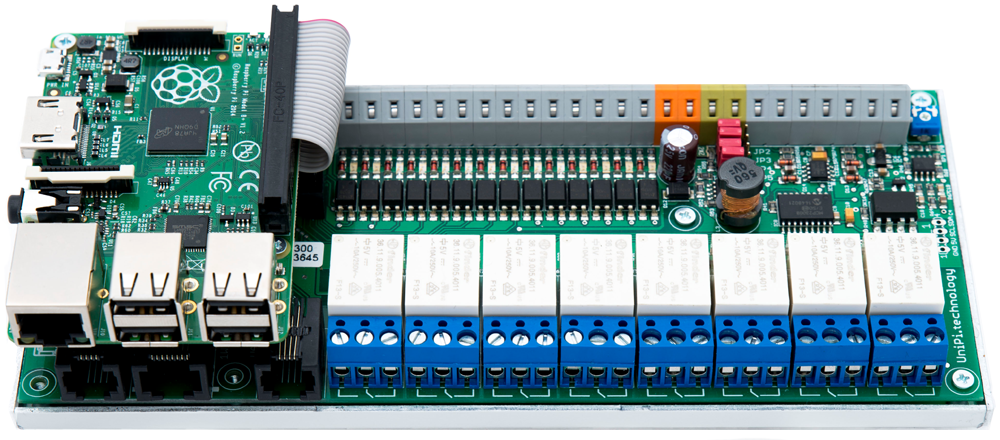
\includegraphics[scale=0.7]{obrazky/unipi_v1}
  \end{center}
  \caption{Popis UniPi v1 \cite{UniPiBoard1}}
\end{figure}

\subsubsection{Popis desky}
\begin{itemize}
	\item 14 digitálních vstupů 5\,–\,24\,V. 
	\item 1Wire sběrnice pro měření teploty a vlhkosti. 
	\item 8 přepínacích relé 250\,V/5\,A AC nebo 24\,V/5\,A DC.
	\item 1 Analogový výstup 0\,–\,10\,V.
	\item 2 Analogové vstupy 0\,–\,10\,V.
	\item Modul reálného času.
	\item I2C sběrnice.
	\item EEPROM paměť.
	\item UART sběrnice.
	\item Notifikační diody pro zobrazení stavu jednotlivých portů.
\end{itemize}

Velkou výhodou řídicí jednotky UniPi je zabudovaný čip pro obsluhu teplotních čidel na sběrnici 1Wire. Digitální teploměry mají svou adresu, není tedy nutné je jakkoliv kalibrovat či nastavovat, stačí zapojit.

S RaspberryPi je deska UniPi propojena 26\,žilovým kabelem přes GPIO konektor. Jak bylo popsáno v kapitole o konektoru GPIO, toto propojení je z důvodu kompatibility shodné pro všechny verze RaspberryPi. Vnitřní uspořádání desky je řešeno pomocí funkčních celků  (obr. \ref{SchemaBlok1}), které jsou propojeny pomocí I2C sběrnice. Výstupy jednotlivých celků jsou poté vyvedeny na konektory desky.
 \begin{figure}[!h]
  \begin{center}
    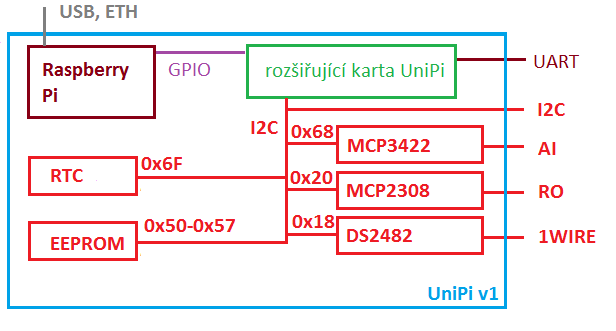
\includegraphics[scale=0.7]{obrazky/unipi_schema1}
  \end{center}
  \caption{Blokové schéma UniPi v1 \colorbox[rgb]{0,1,0}{překreslit}}
	\label{SchemaBlok1}
\end{figure}

Napájení desky je řízeno jumperem JP1 a může být řešeno dvěma způsoby:
\begin{itemize}
	\item Adaptérem 5\,V/2\,A do UniPi, s distribucí 5\,V/750\,mA do RaspberryPi.
	\item Samostatným nápajením obou desek.
\end{itemize}


Pro účely testování a implementace byla zapůjčena deska UniPi s počítačem RaspberryPi 2. Vývoj této desky byl již ukončen a nahrazen druhou verzí, označovanou jako UniPi NEURON.



%%%%%%%%%%%%%%%%%%%%%%%%%%%%%%%%%%%%%%%
%%%%%%%%%%%%%%%%%%%%%%%%%%%%%%%%%%%%%%%
%%%%%%%%%%%%%%%%%%%%%%%%%%%%%%%%%%%%%%%

\section{UniPi v2 - Neuron}
\label{KapitolaUnipi2}

UniPi Neuron představuje modulární PLC (Programmable Logic Controller) pro chytrou domácnost a inteligentní systémy budov, řízení a průmyslovou automatizaci. Díky modulární a kompaktní konstrukci nabízí jedinečnou variabilitu funkcí. UniPi Neuron je univerzální řídící jednotka. Neuron lze použít k řízení chytrého domu nebo jako domácí server. Je vhodný pro monitorování, sběr a ukládání dat na vzdálený server, nebo jako výkonná a plně vybavená brána pro ostatní zařízení \cite{UniPiBoard2}.

 \begin{figure}[!h]
  \begin{center}
    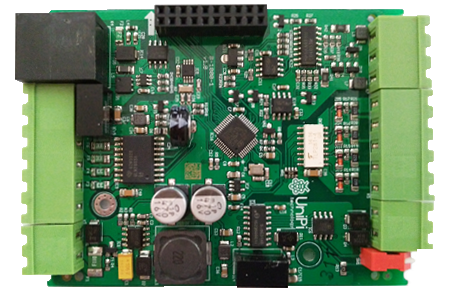
\includegraphics[scale=0.8]{obrazky/unipi_unipi_deska}
  \end{center}
  \caption{UniPi rozšiřující deska \colorbox[rgb]{0,1,0}{vyfotit rovně}}
\end{figure}

UniPi Neuron je na rozdíl od první verze, kdy se rozšiřující deska RaspberryPi distribuovala zvlášt, již hotové řešení, které se skládá z RaspberryPi, rozšiřující desky UniPi verze 2, propojovací desky pro komunikační moduly a diodového panelu. To vše propojené a uzavřené v modrém plechovém pouzdru s možností montáže na DIN lištu. K dostání je tedy pouze jako hotový výrobek.


\subsubsection{Popis desky}
\begin{itemize}
\item Digitalní vstup 4\,-\,24\,V (počet závislý na konkrétním modelu).
\item Transistorový výstup 50V/750 mA(počet závislý na konkrétním modelu).
\item Analog output 0\,-\,10\,V.
\item Analogový vstup 0\,-\,10\,V.
\item 1Wire sběrnice.
\item RS-485 .
\item Modul reálného času.
\item Notifikační diody pro zobrazení stavu jednotlivých portů.
\end{itemize}

UniPi Neuron existuje v několika verzích, odvislých od počtu digitálních vstupů a výstupů, parametrů procesoru a velikosti paměti RAM. Do budoucna by měly být také k dostání verze s jedním konkrétním modulem (WM-Bus, ZigBee, GPRS, \ldots) uvnitř.

\newpage

 \begin{figure}[!h]
  \begin{center}
    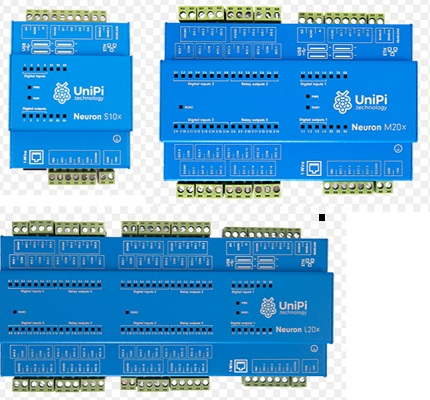
\includegraphics[scale=1.05]{obrazky/unipi_unipi_verze}
  \end{center}
  \caption{UniPi NEURON S, M a L  \cite{UniPiBoard2}}
\end{figure}


Standardní modely NEURON mají proměnlivé množství digitálních vstupů a reléových výstupů. Jejich počet je uveden v Tab.\ref{TableUnipiIO}.



\begin{table}[!ht]
\caption{Porovnání modelů UniPi NEURON dle IO \cite{UniPiBoard2}}
\label{TableUnipiIO}
	\begin{center}
	\begin{tabular}{|l|c|c|c|}
		\hline
		\textbf{Model} & \multicolumn{1}{l|}{\textbf{\begin{tabular}[c]{@{}l@{}}Počet\\ digitálních \\ vstupů\end{tabular}}} & \multicolumn{1}{l|}{\textbf{\begin{tabular}[c]{@{}l@{}}Počet \\ digitálních \\ výstupů\end{tabular}}} & \multicolumn{1}{l|}{\textbf{\begin{tabular}[c]{@{}l@{}}Velikost \\ na DIN liště\end{tabular}}} \\ \hline
		\textbf{S10x} & 4 & 0 & 4 moduly \\ \hline
		\textbf{M10x} & 12 & 8 & 8 modulů \\ \hline
		\textbf{M20x} & 20 & 14 & 8 modulů \\ \hline
		\textbf{M30x} & 34 & 0 & 8 modulů \\ \hline
		\textbf{M40x} & 4 & 28 & 8 modulů \\ \hline
		\textbf{L20x} & 36 & 28 & 12 modulů \\ \hline
		\textbf{L30x} & 64 & 0 & 12 modulů \\ \hline
		\textbf{L40x} & 4 & 56 & 12 modulů \\ \hline
	\end{tabular}
	\end{center}
\end{table}

\newpage

Písmeno x v tabulce (\ref{TableUnipiVar}) bývá nahrazeno číslem 1-3 dle osazeného typu RaspberryPi:

\begin{table}[!ht]
\caption{Varianty modelů UniPi NEURON dle CPU a RAM \cite{UniPiBoard2}}
\label{TableUnipiVar}
	\begin{center}
\begin{tabular}{|c|c|c|c|c|}
\hline
x & \textbf{Osazená deska} & \textbf{CPU} & \textbf{RAM} & \textbf{Další vlastnosti} \\ \hline
\textbf{1} & RaspberryPi B+ & 700\,MHz & 512\,MB &  \\ \hline
\textbf{2} & RaspberryPi 2 & 4x900\,MHz & 1\,GB &  \\ \hline
\textbf{3} & RaspberryPi 3 & 4x1200\,MHz & 1\,GB & BT 4.1, WiFi 802.11n \\ \hline
\end{tabular}
	\end{center}
\end{table}

S RaspberryPi je deska UniPi propojena, obdobně jako u první verze, pomocí 26 pinové desky propoující GPIO port na RaspberryPi s konektorem na rozšiřující desce UniPi. Na samotné propojující desce (Obr.\ref{PicureUniPi1}) je vyvedena UART a I2C sběrnice. 

 \begin{figure}[!h]
  \begin{center}
    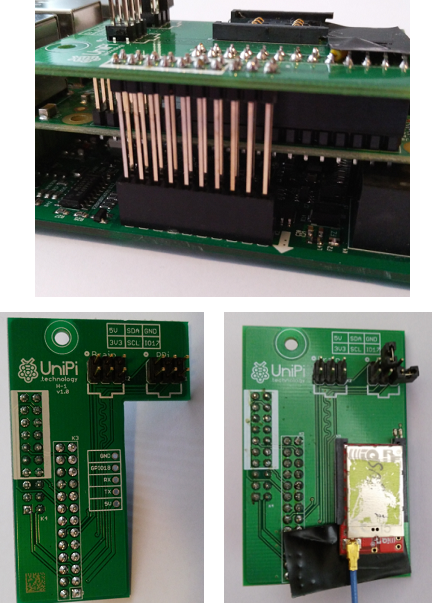
\includegraphics[scale=0.70]{obrazky/unipi_propojbrain}
  \end{center}
	\label{PicureUniPi1}
  \caption{Detail propojovací desky s připojeným WM-Bus modulem \colorbox[rgb]{0,1,0}{přefotit lip}}
\end{figure}

Na I2C sběrnici je nadále připojen panel (Obr.\ref{PicureUniPi2}) se signalizačními diodami. UART sběrnice je zde připravena pro připojenů dalších modulů. Tyto desky jsou k dostání v několika verzích, přizpůsobené konektorem pro konkrétní komunikační modul.

 \begin{figure}[!h]
  \begin{center}
    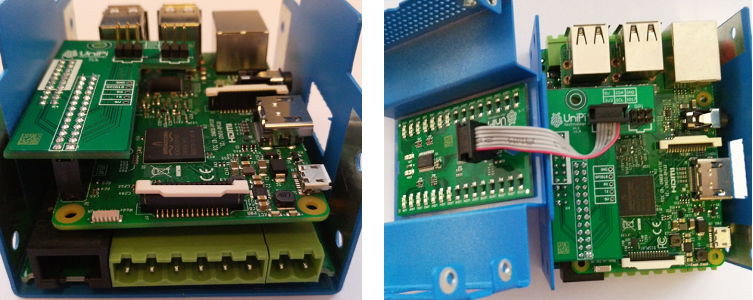
\includegraphics[scale=0.65]{obrazky/unipi_propojuvnitr}
  \end{center}
	\label{PicureUniPi2}
  \caption{Detail vnitřního uspořádání UniPi Neuronu S103 \colorbox[rgb]{0,1,0}{přefotit lip}}
\end{figure}

Vnitřní uspořádání desky je řešeno pomocí funkčních celků (Obr. \ref{BlokSchema2}), které jsou propojeny pomocí I2C sběrnice. Výstupy jednotlivých celků jsou poté vyvedeny na konektory desky.
 \begin{figure}[!h]
  \begin{center}
    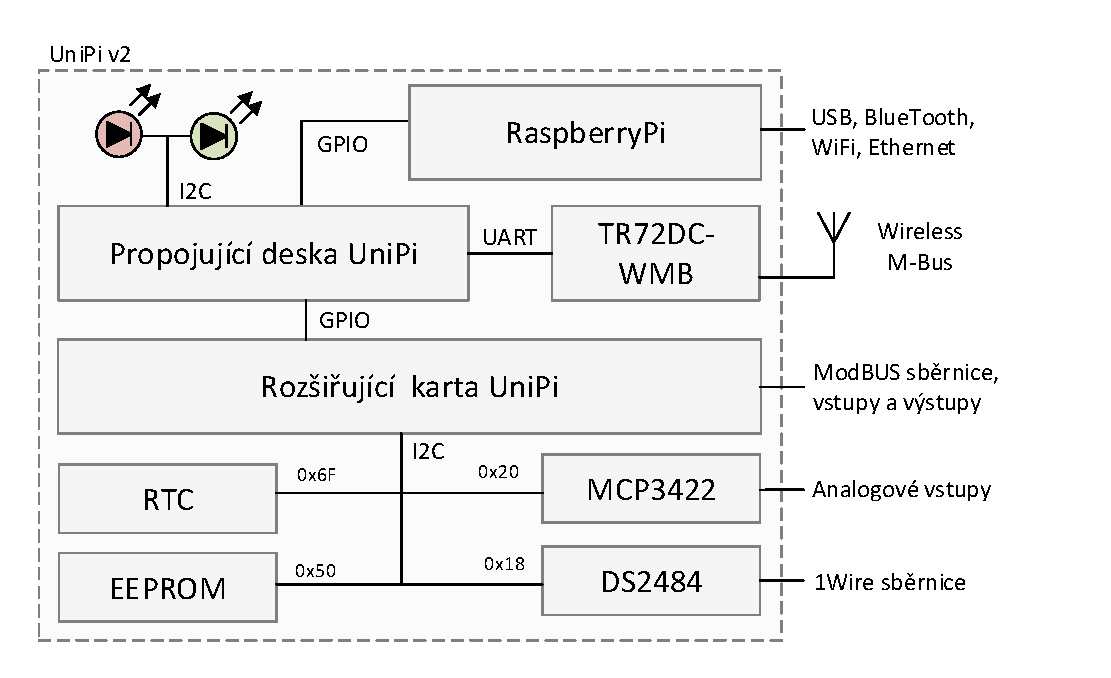
\includegraphics[scale=0.55]{obrazky/unipi_schema2}
  \end{center}
	\label{BlokSchema2}
  \caption{Blokové schéma UniPi v2 \colorbox[rgb]{0,1,0}{překreslit}}
\end{figure}



Napájení desky je pomocí 24\,V/1.5\,A adaptéru přímo na rozšiřující desku UniPi. Pro účely testování a implementace byla zapůjčena deska UniPi Neuron S103 vybavená počítačem RaspberryPi3.

 %\begin{figure}[!h]
 % \begin{center}
 %   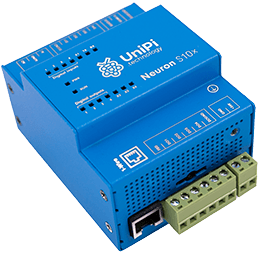
\includegraphics[scale=1.0]{obrazky/unipi_v2}
 % \end{center}
 % \caption{UniPi Neuron S10x (v2) [docasne prevzeti]}
%\end{figure}


 
 


%%%%%%%%%%%%%%%%%%%%%%%%%%%%%%%%%%%%%%%
%%%%%%%%%%%%%%%%%%%%%%%%%%%%%%%%%%%%%%%
%%%%%%%%%%%%%%%%%%%%%%%%%%%%%%%%%%%%%%%

\section{Srovnání obou verzí}

Jak bylo popsáno v předchozím textu (\ref{KapitolaUnipi1},\ref{KapitolaUnipi2}), obě verze UniPi se liší svými parametry a využitím. I když vývoj UniPi byl nahrazen vývojen UniPi NEURONu, stále se najdou aplikace vhodné pouze pro původní desku:


\begin{itemize}
	\item Deska UniPi má reléově spínané výstupy, lze pomocí ní spínat i silové výstupy do 250\,V. Zatímco UniPi NEURON má spínané tranzistorové výstupy pouze do 50\,V, pro spínání vyšších napětí je nutné připojit reléový modul.
	\item Deska UniPi má zpřístupněnou I2C a UART sběrnici, zatímco na UniPi Neuronu je I2C využita pouze pro adresování vnitřních bloků a UART sběrnice je alokována pro rozšiřující komunikační moduly.
	\item Software EVOK a software postavené na něm jsou v tomto okamžiku plně funkční pouze na desce první verze.	
\end{itemize}

Na některé aplikace však již tato deska vhodná není a je lepší využít UniPi NEURON:

\begin{itemize}
	\item I když UniPi první verze má sběrnici UART a teoretecky do ní lze připojit stejné rozšiřující komunikační moduly jako do UniPi Neuronu, součástí vývoje budou jen rozšiřující desky pro UniPi NEURON, jejichž nabídka má obsahovat spoustu dostupných technologií.
	\item Vzhledem k rozsáhlé nabídce modelů UniPi NEURON lze zvolit řešení na míru, včetně další konektivity.
	\item UniPi NEURON disponuje sběrnici RS-485 s protokolem ModBUS.
	\item UniPi NEURON má na kontaktech vysouvací svorky a celý modul zabírá méně místa.	
\end{itemize}

Vzhledem k tomu, že UniPi NEURON je v době vypracování práce jediná vývojem podporovaná verze, bude implementaci WM-Bus protokolu provedena na této verzi, avšak lze bez jakýchkoliv softwarových modifikací a pouze s jednou hardwarovou modifikací implementovat WM-Bus protokol i na UniPi první verze. Stačí pouze propojit příslušné piny IQRF modulu s piny modulárního konektoru UART sběrnice.


%%%%%%%%%%%%%%%%%%%%%%%%%%%%%%%%%%%%%%%
%%%%%%%%%%%%%%%%%%%%%%%%%%%%%%%%%%%%%%%
%%%%%%%%%%%%%%%%%%%%%%%%%%%%%%%%%%%%%%%

\section{Sběrnice na UniPi}
Jak je patrné z předhozích kapitol, jednodeskové počítače i rozšiřující moduly disponují množstvím komunikačních sběrnic. V této kapitole budou stručně představeny všechny výše zmíněné a zaměříme se na sběrnici UART, která bude sloužit pro komunikaci mezi RaspberryPi a WM-Bus modulem.

\subsubsection{UART}
UART je synchronní a asynchronní sériové rozhraní pro přenos dat mezi zařízeními v obou směrech. Používá se pro komunikaci mezi mikrokontroléry, počítači a dalšími zařízeními podporující tento standard. Využívá dvouvodičovou sběrnici, vysílá data na pinu označovaném obvykle jako TX, přijímá na pinu RX.

Pro přenos se používají rámce, které mohou mít 5 až 9 bitů a jsou od sebe odděleny jedním start bitem a jedním nebo dvěma stop bity. Každý rámec může obsahovat ještě paritní bit pro kontrolu rámce. Dále je možné nastavit rychlost přenosu dat od 1 200 bps až do 250 kbps. Lze nastavit buď pro asynchronní režim, označovaný jako SCI, například pro RS-232 či RS-485, anebo pro synchronní režim, běžně označovaný jako SPI.

 \begin{figure}[!h]
  \begin{center}
    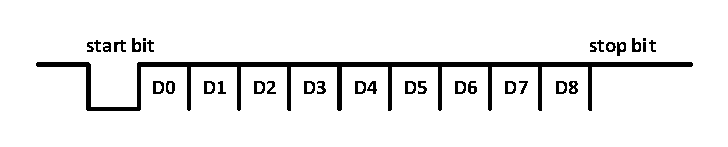
\includegraphics[scale=1.0]{obrazky/sbernice_uart}
  \end{center}
  \caption{UART rámec \cite{sberniceUART} \colorbox[rgb]{0,1,0}{překreslit}}
\end{figure}

Tato sběrnice je ve verzi 1 vyvedená do modulárního konektoru na desce, ve verzi není vyvedená na kontakty, ale je součástí desky plošného spoje, na kterém se přímo nachází slot pro komunikační modul.




\subsubsection{SPI}
SPI je sériové periferní rozhraní. Používá se pro komunikaci mezi řídícími mikroprocesory a ostatními integrovanými obvody. Jednotlivé obvody jsou propojeny čtyřmi vodiči:
\begin{itemize}
	\item Datový výstup MOSI (Master Out, Slave In) obvodu Master je připojen na vstupy MOSI všech obvodů Slave.
	\item Datový vstup MISO (Master In, Slave Out) obvodu Master je propojen s výstupy MISO všech obvodů Slave.
	\item Výstup hodinového signálu SCK je připojen na vstupy SCK všech obvodů Slave.
	\item Každý obvod Slave má vstup SS (Slave Select) pro výběr obvodu.
\end{itemize}
Komunikace je realizována pomocí společné sběrnice, je typu master-slave. Adresace se provádí pomocí zvláštních vodičů, které při logické nule aktivují příjem a vysílání zvoleného zařízení. Tato sběrnice se ani v jedné z desek UniPi nepoužívá ani neni vyvedena ven.

\subsubsection{RS-485}
RS-485 se používá především v průmyslovém prostředí. Vyznačuje se dvouvodičovým propojením jednotek. Tyto vodiče se označují písmeny A a B. Přenos je poloduplexní, a proto se vyžaduje řízení přenosu dat. Pomocí dvouvodičové linky je možné připojit až 32 zařízení. Tato sběrnice není součástí první verze desky, v druhé verzi je vyvedena na kontakty.

\subsubsection{I2C}
I2C je interní datová sběrnice sloužící pro komunikaci a přenos dat mezi jednotlivými integrovanými obvody většinou v rámci jednoho zařízení. Sběrnice je duplexní a dvoudrátová. Na jednu sběrnici může být připojeno více obvodů, v základní sedmibitové verzi až 128 obvodů.
Vodiče jsou označeny jako serial data (SDA) a serial clock (SCL). Sběrnice je typu master-slave. Master při přenosu generuje hodinový signál na vodiči SCL. Když jeden obvod vysílá, všechny ostatní poslouchají a pouze podle adresy určují, zda jsou data určena jim. Obvod, který chce vyslat/přijmout data musí nejprve definovat adresu čipu, s kterým chce komunikovat a zda půjde o příjem nebo vysílání - tedy o čtení nebo zápis. To určuje bit, který je součástí adresy. 

Tato sběrnice je součástí obou verzí desky, využívá se pro propojení vnitřních funkčních bloků (EEPROM, RTC modul, AD převodník, 1Wire master, ...), v první verzi je i vyvedená do modulárního konektoru na desce, v druhé verzi již ne.

\subsubsection{1Wire}
Sběrnice 1Wire, navržená firmou Dallas Semiconductor, umožňuje připojit několik zařízení k řídící jednotce prostřednictvím pouhých dvou vodičů: data a zem. Sběrnice má jeden řídící obvod (master) a jeden či více ovládaných zařízení (slave). Všechny obvody jsou zapojeny jednak na společnou zem, a jednak paralelně na společný datový vodič. Tato sběrnice je součástí obou verzí desky, slouží pro připojení externích čidel (nejčastěji teplotní čidla) a u obou verzí desky je vyvedena do modulárního konektoru.

\subsubsection{GPIO}
\label{KapGPIO}
GPIO jsou piny, které lze programovat pomocí softwaru. Do těchto pinů lze posílat elektrický signál nebo jej z nich naopak přijímat. Na RaspberryPi 1 je takových vývodů celkem 26, na RaspberryPi 2 a RaspberryPi 3 je vývodů 40. GPIO vývodů je zde standardně 8, krom nich se zde nachází i dva piny pro UART, dva pro I2C a šest pro SPI, ty však jdou také přenastavit pro GPIO využití. Nesmíme zapomenout ani na dva výstupy s napětím (3,3\,V a 5\,V) a zem.
Obrázek \ref{ObrazekGPIO} demonstruje rozložení GPIO konektoru napříč verzemi RaspberryPi.

 \begin{figure}[!h]
  \begin{center}
    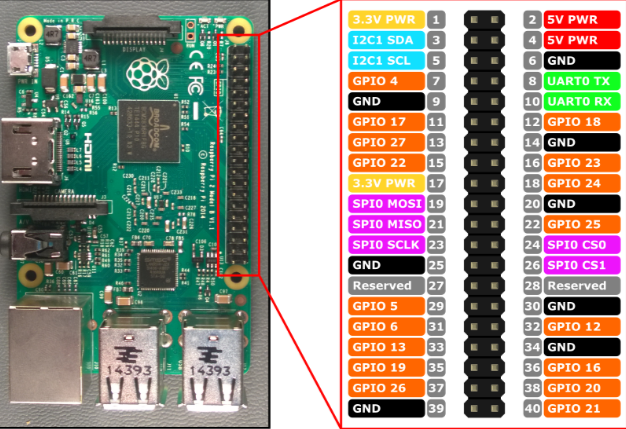
\includegraphics[scale=0.4]{obrazky/sbernice_gpio}
  \end{center}
  \caption{GPIO na RaspberryPi 2 \colorbox[rgb]{0,1,0}{překreslit}}
\end{figure}

 \begin{figure}[!h]
  \begin{center}
    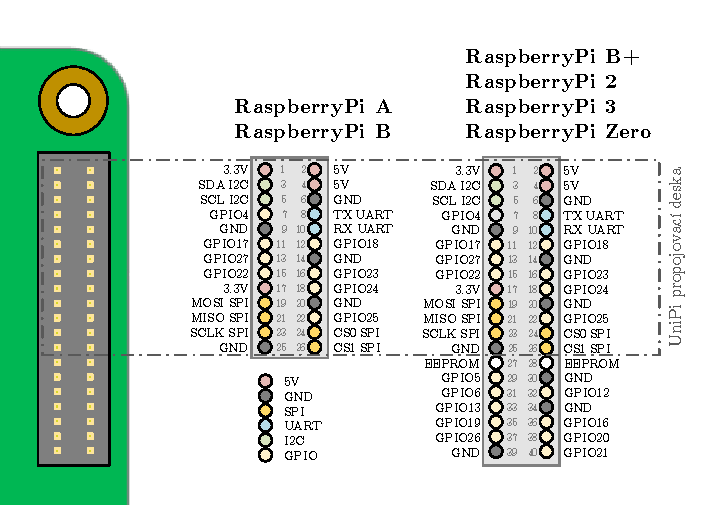
\includegraphics[scale=0.6]{obrazky/unipi_gpio}
  \end{center}
  \caption{Zpětná kompatibilita GPIO konektoru \cite{raspiGPIOs} \colorbox[rgb]{0,1,0}{do tabulky}}
	\label{ObrazekGPIO}
\end{figure}

\newpage 

Jak již bylo popsáno v předchozích kapitolách, GPIO konektor není ve všech verzích RaspberryPi shodný. Model RaspberryPi B má 26 pinový konektor, zatímco verze B+, 2 a 3 mají konektor 40 pinový. Rozdíl je v tom, že u 40 pinového konektoru je prvních 26 pinů shodných a konektor je na zbývajících 14 pinech rozšířen o další vstupy a výstupy. Je tedy zpětně kompatibilní.


%%%%%%%%%%%%%%%%%%%%%%%%%%%%%%%%%%%%%%%
%%%%%%%%%%%%%%%%%%%%%%%%%%%%%%%%%%%%%%%
%%%%%%%%%%%%%%%%%%%%%%%%%%%%%%%%%%%%%%%


\section{Software pro UniPi}

Hlavní výhodou otevřené platformy RaspberryPi je možnost použít zákazníkem zvolený libovolný software. Neexistují omezení ze strany výrobce, proto si může každý svoje řešení postavit na míru.

Výrobce poskytuje vlastní software EVOK, který se stará o komunikaci desky UniPi přes virtuální server či API (Application Programming Interface) s uživatelem. Většina dalších open-source programů využívá toto API pro svůj provoz. Výrobcem je taktéž podporován software Mervis \cite{MervisWeb}, který z UniPi dělá plnohodnotné PLC. Dále je k dipozici několik open-source programů:
\begin{itemize}
\item EVOK - oficiální Python API s websocket a REST podporou.
\item PiDome - platforma pro domácí automatizaci.
\item pimmatic - platforma pro domácí automatizaci založená na node.js.
\item Node-RED - platforma založená na node.js s integrací do společnosti IBM Cloud Bluemix.
\item Wyliodrin - programování automatizace na bázi prohlížeče.
\item FHEM.de - domácí automatizační projekt napsaný v jazyce Perl.
\item JEEDOM - automatizační projekt napsaný v jazyce PHP.
\end{itemize}
A tři komerční:
\begin{itemize}
\item Mervis - profesionální domácí automatizační řešení s on-line SCADA.
\item REX - profesionální PLC s podporou mnoha průmyslových protokolů.
\item HomeSeer - odhlehčená platforma pro automatizaci domácnosti.
\end{itemize}

V době psaní této práce byl EVOK k dispozici i pro druhou verzi desky, avšak bez podpory komunikačních modulů. Implementace protokolu tedy bude prováděna jako samostatná aplikace s vlastní formou vizualizace naměřených dat.





 